% !TeX program = pdflatex
%
% Project Hive -- technical reference (companion to hive_preprint.tex)
% Single-file. Compile with:
%   pdflatex hive_overview.tex
%
\documentclass[10pt]{article}

\usepackage[a4paper, margin=0.8in]{geometry}
\usepackage[T1]{fontenc}
\usepackage[utf8]{inputenc}
\usepackage{amsmath}
\usepackage{amssymb}
\usepackage{booktabs}
\usepackage{tabularx}
\usepackage{array}
\usepackage{microtype}
\usepackage{xcolor}
\usepackage{enumitem}
\usepackage{titlesec}
\usepackage{tikz}
\usetikzlibrary{arrows.meta, positioning}
\usepackage{fancyhdr}
\usepackage[hidelinks]{hyperref}

% ---------------------------------------------------------------- palette
\definecolor{accent}{HTML}{0E6B58}
\definecolor{energy}{HTML}{A8620C}
\definecolor{ghost}{HTML}{8C4157}
\definecolor{ink}{HTML}{131A17}
\definecolor{muted}{HTML}{59635E}
\definecolor{rule}{HTML}{C9D2CD}

\AtBeginDocument{\color{ink}}

\titleformat{\section}
  {\normalfont\normalsize\bfseries\color{accent}}{\thesection\quad}{0pt}{}
  [\vspace{-0.5em}\color{rule}\rule{\textwidth}{0.6pt}]
\titlespacing*{\section}{0pt}{1.0em}{0.4em}

\setlist[enumerate]{itemsep=0.1em, topsep=0.15em, leftmargin=1.3em}
\setlist[itemize]{itemsep=0.1em, topsep=0.15em, leftmargin=1.0em}

\newcolumntype{L}{>{\raggedright\arraybackslash}X}

\newcommand{\code}[1]{\texttt{\small #1}}
\newcommand{\note}[1]{\par\vspace{0.15em}{\footnotesize\color{muted}#1}\par}
\newcommand{\tabhead}[1]{\textbf{#1}}

\pagestyle{fancy}
\fancyhf{}
\renewcommand{\headrulewidth}{0pt}
\fancyfoot[L]{\footnotesize\color{muted}Project Hive --- Technical Reference}
\fancyfoot[C]{\footnotesize\color{muted}Phase 1}
\fancyfoot[R]{\footnotesize\color{muted}\thepage}

\setlength{\parindent}{0pt}
\setlength{\parskip}{0pt}

\begin{document}

% ---------------------------------------------------------------- masthead
{\LARGE\bfseries Project Hive}\hfill{\footnotesize\color{muted}\textsc{Technical Reference} $\cdot$ Phase 1 $\cdot$ \today}\\[0.3em]
{\color{muted}\small One fine-tuned Qwen3-4B, driven as a colony; a non-model orchestrator owns all state, energy, and lifecycle. Target: single 16\,GB T4.}\\[0.45em]
\color{ink}\rule{\textwidth}{1pt}
\vspace{0.6em}

\resizebox{\textwidth}{!}{%
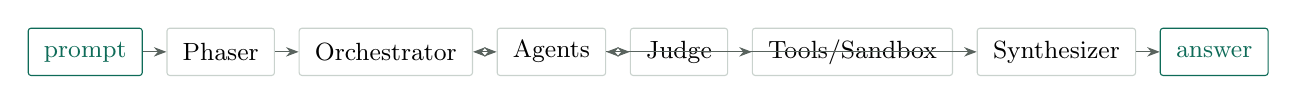
\begin{tikzpicture}[
  box/.style={draw=rule, rounded corners=1pt, align=center, font=\small,
              minimum height=6mm, inner xsep=2mm},
  hum/.style={box, draw=accent, text=accent},
  >={Stealth[length=1.6mm]}
]
\node[hum] (in) {prompt};
\node[box, right=3mm of in]  (ph)  {Phaser};
\node[box, right=3mm of ph]  (orc) {Orchestrator};
\node[box, right=3mm of orc] (ag)  {Agents};
\node[box, right=3mm of ag]  (jd)  {Judge};
\node[box, right=3mm of jd]  (tl)  {Tools/Sandbox};
\node[box, right=3mm of tl]  (sy)  {Synthesizer};
\node[hum, right=3mm of sy]  (out) {answer};
\draw[->, muted]  (in)  -- (ph);
\draw[->, muted]  (ph)  -- (orc);
\draw[<->, muted] (orc) -- (ag);
\draw[->, muted]  (ag)  -- (jd);
\draw[<->, muted] (ag)  -- (tl);
\draw[->, muted]  (jd)  -- (sy);
\draw[->, muted]  (sy)  -- (out);
\end{tikzpicture}}

\vspace{0.5em}
\begin{tabularx}{\textwidth}{@{}l r L@{}}
\toprule
\tabhead{Module} & \tabhead{LOC} & \tabhead{Owns} \\
\midrule
\code{main.py}            & 204  & Object construction, dependency injection \\
\code{problem\_phaser.py} & 441  & Prompt $\to$ spec; complexity score; energy budget \\
\code{orchestrator.py}    & 1014 & Tick loop, event routing, spawn/promote/kill \\
\code{agent\_node.py}     & 938  & \code{think}/\code{decide}/\code{execute} \\
\code{task\_graph.py}     & 211  & DAG, dependency gating, cycle detection \\
\code{colony\_state.py}   & 160  & Agent registry, energy ledger \\
\code{judge.py}           & 409  & Three-tier verification \\
\code{ghost\_extractor.py} & 150 & Dead agent $\to$ JSON-serialisable failure record \\
\code{memory\_state.py}   & 201  & \code{MemoryStore}; two FAISS indices (ghost, success) \\
\code{synthesizer.py}     & 155  & Final decode \\
\code{tools.py}           & 1424 & Tool router, sandbox, resource limits (was 1291 pre-patch) \\
\bottomrule
\end{tabularx}
\note{12 modules, 5{,}370 lines post-patch (exact, re-counted with \code{wc -l} against the patched tree). \textbf{\code{main.py} does not run as committed} --- it is Kaggle-notebook cells concatenated with every import commented out. This precedes every bug below it in this document: nothing downstream is even reachable until \code{main.py} is made runnable, independent of whether \code{memory\_state.py:30} is also fixed.}

% ================================================================== SECURITY
\section{Sandbox security review}

\code{run\_code} executes agent-supplied Python as a real OS subprocess
(\code{sys.executable} on a temp script, no chroot/namespace/seccomp). Everything
below the line is enforced entirely in-process by prepended Python preambles;
there is no OS-level isolation backstop. Two vulnerabilities were present in the
committed code and are fixed below; a third defect (unrelated to security)
silently broke \code{run\_code} on Windows entirely.

\vspace{0.4em}
\begin{tabularx}{\textwidth}{@{}l L@{}}
\toprule
\tabhead{Vuln} & \tabhead{Unrestricted filesystem I/O inside \code{run\_code}} \\
\midrule
Vector & Network, process-spawn, and \code{importlib.reload} were gated; plain \code{open()}/\code{os.remove}/\code{shutil.rmtree} were not. Agent code had full read/write/delete of anything the host OS user could reach --- SSH keys, other users' files, host source --- entirely outside \code{SAFE\_READ\_ROOT}/\code{SAFE\_WRITE\_ROOT}. \\
Exfil path & \code{run\_code}'s stdout is returned directly to the calling agent (and from there, the model): \code{print(open(path).read())} required no network access at all. \\
Fix & \code{FILE\_GATING\_PREAMBLE} wraps \code{builtins.open}/\code{io.open}/\code{os.open}; each call resolves the target's \code{realpath} and rejects anything outside the sandbox's own ephemeral \code{TemporaryDirectory} cwd (read/write) or \code{SAFE\_READ\_ROOT} (read-only --- needed so \code{query\_dataframe}'s sandboxed \code{pd.read\_csv} can still reach its pre-vetted target). \code{os.remove}/\code{unlink}/\code{rmdir}/\code{rename}/\code{replace}/\code{shutil.rmtree}/\code{move} are blocked outright: the sandbox dir is discarded every run, so agent code has no legitimate use for them, and a containment check on a delete is one TOCTOU race from a delete-anything primitive. \\
\bottomrule
\end{tabularx}

\vspace{0.4em}
\begin{tabularx}{\textwidth}{@{}l L@{}}
\toprule
\tabhead{Vuln} & \tabhead{Full host environment inherited by the sandbox subprocess} \\
\midrule
Vector & \code{subprocess.Popen(...)} carried no \code{env=}, so it inherited the orchestrator process's entire environment by default --- any HF token, API key, or cloud credential the host held. \\
Exfil path & \code{print(dict(os.environ))} inside \code{run\_code}, returned verbatim on stdout. Zero network calls required, same channel as above. \\
Fix & \code{SANDBOX\_ENV} is now an explicit allow-list (\code{PATH}, \code{SYSTEMROOT}, \code{TEMP}, \code{TMP}, \code{PYTHONIOENCODING}) passed as \code{env=} to \code{Popen}. Nothing the host process held secrets in survives into the child. \\
\bottomrule
\end{tabularx}

\vspace{0.4em}
\begin{tabularx}{\textwidth}{@{}l L@{}}
\toprule
\tabhead{Defect} & \tabhead{\code{run\_code} crashed on every call on Windows (pre-existing, non-security)} \\
\midrule
Cause & Sandbox script was written with \code{open(path, "w")} --- no encoding, so Windows defaulted to \code{cp1252}. The existing network/process-gate preambles use box-drawing characters (\code{──}) in comments, unencodable in \code{cp1252}: every call raised \code{UnicodeEncodeError} before the subprocess ran. \\
Fix & \code{encoding="utf-8"} pinned on the write, matching how stdout/stderr are already decoded. \\
\bottomrule
\end{tabularx}
\note{General lesson: any file write whose content is not guaranteed ASCII must pin an explicit encoding rather than inherit the platform default, or the failure is silent on the platform the code ships to even when it never surfaces on the platform it was written on. The full preprint (Section 3.5) documents an analogous case: an agent-supplied timeout that flowed unvalidated into \code{subprocess.communicate()} ran for roughly eleven days before external termination --- both bugs are instances of the same rule, that any parameter or content a model or platform can vary must be validated or normalised at the boundary, not assumed.}

\vspace{0.4em}
\begin{tabularx}{\textwidth}{@{}l l@{}}
\toprule
\multicolumn{2}{@{}l}{\tabhead{Sandbox layer stack} (subprocess, applied in order)} \\
\midrule
network gating         & socket/DNS blocked, C-level (\code{\_socket}) and subclass patched \\
process-spawn gating   & subprocess/os/\code{\_posixsubprocess}/\code{\_winapi}/ctypes dlopen blocked \\
\textcolor{ghost}{\bfseries filesystem gating (new)} & open/os.open jailed to sandbox cwd + read-only \code{SAFE\_READ\_ROOT}; delete/rename blocked \\
module-reload gating   & \code{importlib.reload} blocked (patches survive) \\
domain preamble        & e.g.\ \code{Decimal} precision for math/finance domains \\
\code{RLIMIT\_AS} / \code{RLIMIT\_CPU} & 1\,GB / $2\times$ effective timeout; soft limit set equal to hard limit, so sandboxed code cannot raise its own ceiling back up \\
\textcolor{ghost}{\bfseries env allow-list (new)} & \code{Popen(env=SANDBOX\_ENV)}, no host secrets inherited \\
output capture cap     & 1\,MB/stream, reader threads, kills on overflow \\
process-group kill     & SIGTERM $\to$ escalate SIGKILL, \code{setsid} \\
\bottomrule
\end{tabularx}
\note{\textbf{Gate order.} Mostly incidental --- network, process, file, and reload gates patch disjoint namespaces and can be applied in any relative order, since none is reachable until agent code (appended last) actually runs. One ordering \emph{is} load-bearing, pre-existing and unchanged by this patch: \code{RLIMIT\_AS} is applied \emph{after} the domain preamble, so the 1\,GB cap never chokes a domain preamble's own imports (e.g.\ pandas/numpy) before agent code is reached.}

\note{\textbf{What was actually checked (methodology, not just a conclusion).} (a) \code{tests/test\_tools\_security.py}, the pre-existing suite, 58 tests / 6 skipped / 0 failed, run via \code{pytest tests/test\_tools\_security.py} against the patched tree. (b) Five targeted PoCs run against the live patched sandbox, not the test suite: \code{open()} on an absolute host path outside both allowed roots (blocked, \code{PermissionError}); write+read of a file within the sandbox's own cwd (succeeds, confirms the jail isn't over-broad); \code{os.remove()} on an absolute host path (blocked); a planted \code{HIVE\_TEST\_SECRET} env var read via \code{os.environ} and printed (does not appear in returned stdout); \code{socket.create\_connection} to an external host (blocked, confirms no regression on the pre-existing network gate). All five were re-run after the fix and pass; none is a formal red-team exercise, and none of it substitutes for OS-level sandboxing.}

\note{\textbf{Known open gaps, not mitigated --- not filed as out-of-scope.} \code{del sys.modules['socket']} followed by re-import reaches the same restore-the-real-module effect as \code{importlib.reload} without calling \code{reload} itself, and it is plain Python: \emph{exactly} the code path \code{run\_code} already lets agent-supplied code execute, not a privileged capability. This is a live bypass of the network/process/file gates for any agent that discovers it, not a residual risk outside the threat model. \code{write\_file}'s output path is \code{SAFE\_WRITE\_ROOT/\{agent\_id\}\_\{basename(filepath)\}} --- both components are supplied by the calling agent within the same colony session, so the full path is attacker-predictable in advance, not merely theoretically guessable; a second, colluding agent that pre-plants a symlink at that exact path before the first agent's \code{write\_file} call would bypass the jail, since \code{open(path,'w')} follows an existing symlink. The current \code{os.path.islink} pre-check narrows but does not close this --- it is check-then-use, and a race between the check and the open is exactly what TOCTOU means. Neither gap has a fix in this patch. Both require, and are deferred to, OS-level isolation (namespace/seccomp) rather than a further in-process patch, since both bypasses operate below the layer an in-process monkeypatch can see.}

% ================================================================== rest
\section{Control flow, budget, verification}

\code{Orchestrator.tick()}, fixed order: (1) energy check --- $\le 5$ halt,
$\le 10$ consolidate; (2) deadlock watchdog, timeout $= 30\text{s}\times$
tickable agents; (3) drain mailbox, route events; (4) dispatch tasks at
\code{in\_degree==0}; (5) tick live agents (\code{think}$\to$\code{decide}$\to$\code{execute}); (6) halt on root
\code{status==2}. Agents never call the orchestrator directly --- only post to
the mailbox.

Budget: $S = \mu(d)\cdot\min(1+0.5\sqrt n,\,2.5)\cdot(1+0.8(1-\cos(g,c)))$, domain
multiplier $\mu \in [1.0, 2.0]$, clamped to $[1,9]$, interpolated to a
100--3000 budget over tiers S/M/L/XL.

\begin{tabularx}{\textwidth}{@{}c L l l@{}}
\toprule
\tabhead{Tier} & \tabhead{Check} & \tabhead{Cost} & \tabhead{Runs} \\
\midrule
\textcolor{accent}{1} & syntax/shape/emptiness & sub-ms & always \\
\textcolor{accent}{2} & cosine vs.\ goal embedding, warn $\le 0.60$, execute $\le 0.30$, 3-strike & 1 dot product & embeddings present \emph{and} output $>$12 words \\
\textcolor{accent}{3} & LLM critique of engagement (last verdict line wins) & full generation & promotion only \\
\bottomrule
\end{tabularx}
\note{Two independent gates on tier 2, not one: \emph{embeddings present} is structural (Phase 1 has no embedding pipeline for some output types); \emph{$>$12 words} is a signal-quality floor (a terse correct answer and a terse wrong answer sit at similar cosine distance from the goal embedding, so similarity carries no signal below that length). Either gate alone skips tier 2; this doc's earlier draft collapsed them into one cell and lost that distinction.}

Energy: spawn decomposer 4, executor/verifier 2; reasoning
\code{max(1,$\Delta$chars//100)}/tick. Stressed $\le10$, death $\le5$. Fan-out
capped independently (root 3, non-root 2) --- \emph{that} cap, not the budget,
bounds concurrent KV caches. Ghost records (role, task, failure type,
deduped/capped reason) persist to FAISS across sessions; success cache is
session-only (0.45 threshold).

\note{\code{RLIMIT\_AS}'s 1\,GB figure (Section~2) is chosen, not profiled: it was not derived by measuring a legitimate \code{query\_dataframe} workload against \code{QUERY\_FILE\_MAX\_BYTES} (100\,MB on disk). A CSV near that on-disk ceiling can plausibly exceed 1\,GB once parsed into a pandas DataFrame with Python object overhead, which would clip a legitimate query rather than only a memory-bomb attack. This has not been tested against a representative large file; treat 1\,GB as a placeholder pending that measurement, not a validated bound.}

% ================================================================== defects
\section{Known defects}

Two axes, not one: \tabhead{Sev.} is blast radius (does the system run at
all, and does it run correctly); \tabhead{Class} is bug (an implementation
mistake with a well-defined fix) versus gap (a capability the architecture
does not yet have, no bug to point at). The text-transport item is filed
\emph{Gap}, not \emph{Design}, deliberately: the full preprint's Section 4
treats replacing it with KV-cache passing as close to the paper's central
architectural bet, not a peer of sibling-task addressability.

\begin{tabularx}{\textwidth}{@{}l l l L@{}}
\toprule
\tabhead{Sev.} & \tabhead{Class} & \tabhead{Location} & \tabhead{Effect} \\
\midrule
\textcolor{ghost}{\bfseries Blocking} & Bug & \code{main.py} & Not runnable as committed --- every import commented out (Kaggle-cell artifact). Precondition for reaching every bug below; listed first because nothing else is reachable until this is fixed. \\
\textcolor{ghost}{\bfseries Blocking} & Bug & \code{memory\_state.py:30} & \code{embedding\_dim = embedding\_dima} --- \code{NameError} on every \code{MemoryStore} construction; kills the run at \code{MemoryStore()} time, before \code{main.py} even reaches the orchestrator. \\
\textcolor{energy}{\bfseries Silent} & Bug & \code{colony\_state.py} & \code{consolidate\_idle\_agents()} checks \code{status=="idle"}, never set. MERGE is a permanent no-op. \\
Moderate & Gap & \code{orchestrator.py} & Sibling task IDs unaddressable within one SPAWN batch. \\
Moderate & Gap & \code{event\_queue.py} & Inter-agent transport is text: decode, truncate to 500 chars, re-tokenise --- the mechanism the full preprint's cache-splicing result (Section~4) is proposed to replace. \\
\bottomrule
\end{tabularx}

\note{\textbf{Reconciling this table with the full preprint's Section 5 (``silent subsystem loss'').} These are two different bugs in two different files, not one bug described two ways. The preprint recounts a \emph{historical} defect in \code{ghost\_extractor.py}: a live GPU tensor leaking into a ghost record made every \code{json.dump()} on write fail, silently swallowed by a try/except, so ghost persistence appeared to run but never actually wrote a record --- already fixed in the code as committed (\code{ghost\_extractor.py} now explicitly discards the tensor field before returning). The \code{memory\_state.py:30} bug above is a separate, currently unfixed defect one layer upstream: it prevents \code{MemoryStore} from constructing at all, which means the already-fixed \code{ghost\_extractor.py} code is never even reached. Sequentially: fix \code{main.py} $\to$ fix \code{memory\_state.py:30} $\to$ only then does the already-fixed \code{ghost\_extractor.py} logic get exercised for the first time.}

\vspace{0.5em}
\color{rule}\rule{\textwidth}{0.6pt}\\[0.3em]
{\footnotesize\color{muted}\url{https://github.com/arkapravopal04/Swarm_neural_nets}}

\end{document}
